%!TEX root = ../thesis.tex
\begin{savequote}[75mm]
Nulla facilisi. In vel sem. Morbi id urna in diam dignissim feugiat. Proin molestie tortor eu velit. Aliquam erat volutpat. Nullam ultrices, diam tempus vulputate egestas, eros pede varius leo.
\qauthor{Quoteauthor Lastname}
\end{savequote}

\chapter{Jira and Confluence: the essentials}

Now that we have understood the concept of Agile, let's get to know the Jira and Confluence, the software used to implement it.
These are proprietary tools are developed and maintained by the Australian company Atlassian.

\begin{figure}[H]
	\centering
	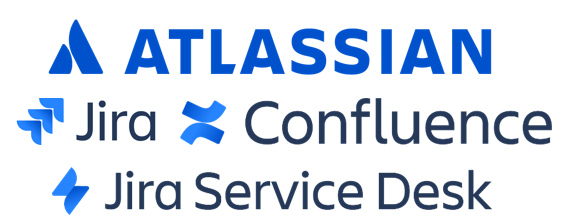
\includegraphics[width=.7\textwidth]{resources/atlassian_logo}\\
	\caption{The logos of \textit{Atlassian}, \textit{Jira}, \textit{Confluence} and \textit{Jira Service Desk}}
\end{figure}

Jira is a proprietary Issue Tracking System that was first released in 2002, this product's name is a truncation of Gojira, the Japanese word for Godzilla.
This is a reference to another ITSs that was dominating the market at the time, Bugzilla.
% https://www.workzone.com/blog/jira-alternatives/
Now the competitors of Jira are other software like, for example, Redmine, VersionOne, PivotalTracker, Workzone or integrated ITSs in repositories like GitHub's or GitLab's issue trackers.
Athonet's previous choice was Redmine because it's open source (this implies it's free of commision), it has a medium large community of people that use it and maintain it behind and the plugins allow the integration with other tools used internally like repositories or software for reporting customer requests, for example.

\begin{figure}[H]
	\centering
	
\includegraphics[width=.6\textwidth]{resources/redmine_logo}\\
	\caption{\textit{Redmine}'s logo}
\end{figure}

Confluence, on the other hand, is designed as a collaboration platform for sharing knowledge like internal documents, product specifications, meeting notes and can be used as an internal wiki for the company and even for the public.
Atlassian released the first version of Confluence in 2004, saying its purpose was to build ``\textit{an application that was built to the requirements of an enterprise knowledge management system, without losing the essential, powerful simplicity of the wiki in the process}''.
%https://en.wikipedia.org/wiki/Confluence_(software)

Since the first releases of these products, Atlassian has developed and acquired new tools like Bamboo, Clover, Crowd, Crucible, and FishEye, all orientated towards collaboration, content sharing, issue tracking, time scheduler, etc.

Both Jira and Confluence are written in Java.

\section{Understanding what they can do}
These tools are made to be integrated with one another, not only because they are made by the same company but they are strictly correlated.
Integrating an issue tracker with a platform able to share documents and thoughts allows a more granular analysis of the problem.
This means that in the company they can store meeting notes and documents related to the project in Confluence, then convert them to Issues in Jira.

Even though there is a license to pay to use these tools it is worth it.

Plugins can extend by far the usage and integration with other tools and the Atlassian Marketplace is full of them.

Let's understand them better.
	
	\subsection{Jira}
	
		Over the years Jira has become such a big software that Atlassian had to separate it in three different components, each with it's own scope.
		A more complete comparison can be found at 
		%http://www.akeles.com/what-are-the-differences-between-jira-software-jira-service-desk-and-jira-core/
	
		%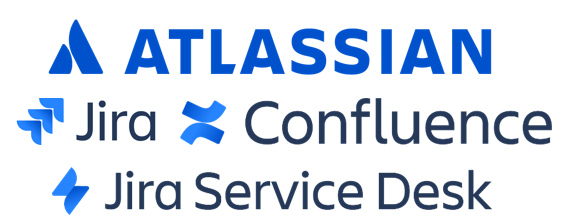
\includegraphics[height=\fontcharht\font`\B]{resources/atlassian_logo} 
		%todo aggiungere piccolo logo dei progetti vicino a ciascun titolo
		\subsubsection{Jira Core}
			Jira Core's main purpose is to handle business processes. 
			It is designed to
			
		\subsubsection{Jira Software}
			Jira Software's main purpose is to ho handle software projects
		
		\subsubsection{Jira Service desk}
			Jira Service desk's main purpose is to handle customer requests

		%https://marketplace.atlassian.com/apps/1212136/portfolio-for-jira/version-history
		\subsubsection{Jira Portfolio Plugin}
			Jira Portfolio was first designed as a plugin from ... then it was acquired by atlassian becaues
			It's main purpose is to visualize project roadmaps
		
	\subsection{Confluence}
		As described earlier, Confluence is a collaboration platform.
		It allows to create spaces of different categories that can be associated with Jira projects.

\section{Key concepts for Jira}
%https://www.atlassian.com/software/jira/guides/getting-started/overview#key-terms-to-know

%todo unificare questi 2 prossimi paragrafi
\section{How they can satisfy Athonet's needs}

	Athonet has chose Atlassian's Jira and Confluence because... 

	The most important feature they needed was the roadmap and allowing this to be easily integrated with the other tools.
	
	The roadmap is a key element for a company, specially for a software one, since it allows to tenere d'occhio release / andamento del progetto

	Con i tool attuali non è possibile avere una tale visione dei progetti
	
	Un altro grande vantaggio di questi tool inoltre è quello di poter avere una wiki centralizzata (adesso sono utilizzati altri tool)

\section{How will Athonet use these tools}

	These tools are very complex, it is necessary to understand the scenario they can be used in and how the

	\subsection{Development} 
		Better tracking of inte
	
	\subsection{Management} 
		A
	
	\subsection{Client interaction} 
		A
		
	\subsection{Internal documentations}
		To be used as a wiki containing all the information for the employees
		
	\subsection{The difference between these and other internal tool}
		Sharepoint, otrs, office 365
		
		impossibile sostituire certi tool come word per la creazione di documenti per la condivizione con clienti / utenti ma sì per documentazione e wiki interna

riprendere necessità dell'azienda\\
fare un paio di uml con le varie figure aziendali e con cosa si andranno ad interfacciare

\section{The Atlassian Community}
	Choosing Jira and Confluence over other tools and implementing a brand new solution aka internally built software (reinventing the wheel) 
	because of the large community behind these tools.
	Atlassian offers a dedicated blog for Q\&A
	There are projects open in Jira online dedicated for Jira and Confluence, allowing users to open tickets and request for new features, report bugs etc.
	This allowed me to find information faster and 
	
	
	EXAMPLES OF COMPANIES THAT USE JIRA AND CONFLUENCE 
	CANONICAL
	+ QUELLA CHE TI HA MANDATO FABIO
